\chapter{Metodologia e Resultados Experimentais}
\label{sec:metodologia}

A condução deste trabalho segue uma abordagem estruturada em três etapas principais: levantamento de dados, modelagem matemática do problema e experimentação por meio de resolvedores matemáticos. A seguir, descrevemos cada uma dessas fases em detalhes.

\section{Levantamento de Dados e Cenários}

Inicialmente, realizou-se o levantamento dos principais parâmetros e cenários utilizados nos modelos de coleta de dados assistida por VANTs, conforme apresentado em trabalhos como \cite{wei2022survey,messaoudi2023survey,liu2018uavWSN}. São coletadas informações sobre os modos de coleta (voo pairado, sobrevoo e híbrido), características dos sensores, limitações energéticas dos VANTs, padrões de cobertura, e tipos de topologia das redes de sensores sem fio.

Além disso, definiu-se o cenário base da simulação, como a área de cobertura, número e distribuição dos sensores, tipo de VANT (asa fixa ou rotativo), tempo máximo de voo e parâmetros de consumo energético. Esses dados são utilizados como entrada para a etapa de modelagem matemática.

\section{Modelagem Matemática}

Com os dados obtidos, foi formulado o modelo matemático para o problema de coleta de dados por VANTs. O problema é estruturado como uma variante de roteamento com restrições energéticas, inspirado em modelos de roteamento capacitado~\cite{toth2002vrp} e em problemas de cobertura com múltiplos alvos~\cite{church1974maximal}.

A função objetivo pode ser definida como a minimização da energia total consumida ou da idade média da informação (AoI), sujeita a restrições de:

\begin{itemize}
\item capacidade energética dos VANTs (Equação~\eqref{eq:energia-capacidade}),
\item cobertura total ou parcial dos sensores (Equação~\eqref{eq:y-visita}),
\item tempo máximo de missão (Equação~\eqref{eq:mov-base}),
\item conectividade entre pontos de coleta e retorno à base (Equação~\eqref{eq:mov-fluxo}).
\end{itemize}

Com base em modelos da literatura, como em \cite{liu2018uavWSN} e \cite{zhang2018drlrvc}, variáveis contínuas e binárias são utilizadas para representar trajetórias, coleta de dados e consumo energético. O modelo é resolvido usando programação inteira mista (MILP).

\section{Testes e Validação com Resolvedor}

A fase final consiste na implementação da modelagem matemática em linguagem compatível com o resolvedor Gurobi, por meio de scripts em Python. Os testes computacionais visam avaliar o desempenho do modelo em diferentes cenários, variando parâmetros como o número de sensores, alcance de comunicação e número de VANTs.

São analisadas as seguintes métricas:

\begin{itemize}
\item energia total consumida por missão,
\item tempo de cobertura dos sensores,
\item distância percorrida,
\item quantidade de sensores visitados.
\end{itemize}

\subsection{Cenários}
Os experimentos foram conduzidos sobre um conjunto de cenários sintéticos que variam dois parâmetros independentes: quantidade de sensores implantados na área de monitoramento e o tamanho da área coberta. Para a quantidade de sensores, foram considerados os valores $n_s \in \{5, 10, 15, 20, 25, 30\}$, e para a dimensão da área quadrada, foram adotados os seguintes tamanhos para o lado do quadrado: $L \in \{100, 200, 400, 600, 800, 1000\}$ metros. A combinação fatorial desses dois parâmetros resulta em 36 cenários distintos, denominados $P_{n_s\text{-}L}$ (ex.: $P_{10\text{-}400}$ para 10 sensores em área de 400×400 m).

Para cada cenário, as coordenadas $(x, y)$ dos sensores são geradas aleatoriamente e distribuídas de forma uniforme dentro da área quadrada de lado $L$, sendo fixadas em arquivos CSV para garantir reprodutibilidade. O posicionamento é mantido constante ao longo de todas as rodadas de simulação, de modo a isolar os efeitos da variação de escala sobre as métricas de desempenho.

Cada cenário é executado por 30 rodadas consecutivas, simulando missões periódicas do VANT. Em cada rodada:

\begin{enumerate}
\item O estado de idade da informação (AoI) de todos os sensores é carregado do estado persistido pela rodada anterior, iniciando em zero na primeira rodada
\item O modelo de otimização é resolvido com horizonte temporal de 20 \textit{slots} de 10\,s (missão de 200\,s), com limite de tempo de 60\,s e tolerância de otimalidade de 1\% (\textit{MIPGap}). 
\item O VANT parte da base, paira sobre os sensores selecionados para coleta e retorna à base.
\item O estado de AoI é atualizado: sensores visitados têm AoI zerada, e os demais acumulam $+1$ por \textit{slot} sem visita.
\end{enumerate}
 

Ao término das 30 rodadas, o estado de AoI é descartado, garantindo independência entre execuções de cenários distintos. 

Após a execução de todos os cenários, os resultados são agregados calculando-se a média das 30 rodadas para cada combinação $(n_s, L)$. Os valores médios são analisados por meio de:
                                                                         
\begin{itemize}
\item \textbf{Gráficos de linha}: evolução de cada métrica em função do tamanho do mapa, com uma curva por quantidade de sensores.
\item \textbf{Mapas de calor}: visualização bidimensional da métrica em função do par $(n_s, L)$, permitindo identificar regiões de maior e menor custo operacional.
\end{itemize}

Duas métricas de AoI são acompanhadas e não devem ser confundidas. A \emph{AoI coletada} é a soma das idades zeradas nas coletas ao longo da missão, ou seja, mede quanta informação desatualizada o VANT efetivamente recolheu (quanto maior, melhor). Já a \emph{AoI média final} é a idade que \emph{resta} nos sensores ao término da missão, calculada como a média, sobre todos os sensores, do número de slots decorridos desde a última coleta de cada um. Ela mede quão desatualizado ficou o conjunto de dados da rede ao final do plano de voo: quanto menor, mais recentes são as informações disponíveis. Enquanto a AoI coletada premia recolher muita informação, a AoI média final penaliza deixar sensores sem visita.



Os resultados obtidos são analisados quantitativamente, com referência aos padrões observados em trabalhos relacionados~\cite{wei2022survey,messaoudi2023survey}, com o objetivo de explorar a sensibilidade do modelo a diferentes configurações de cenário.

\subsection{Configuração dos Drones}

Os experimentos foram conduzidos com dois modelos distintos de VANT, cujos parâmetros físicos alimentam o modelo de potência de asa rotativa (Equação~\eqref{eq:potencia}). Cada modelo dá origem a um conjunto de experimentos sobre os mesmos 36 cenários, descritos a seguir.

\subsubsection{DJI Matrice 300 RTK}
O primeiro conjunto de experimentos utiliza os parâmetros físicos do DJI Matrice 300 RTK, um drone de uso profissional amplamente empregado em aplicações industriais e de monitoramento. Para estes experimentos, a capacidade de bateria foi fixada em $E^{\max} = 2$\,MJ, representando uma fração da autonomia total do veículo com o objetivo de avaliar o comportamento do otimizador em condições mais restritivas de energia.

\subsubsection{Parrot Anafi USA}
O segundo conjunto de experimentos foi realizado com os parâmetros do Parrot Anafi USA, um drone compacto voltado para aplicações de segurança e mapeamento. Para este modelo, a capacidade de bateria utilizada foi $E^{\max} = 141.372$\,J, correspondendo à capacidade real da bateria do equipamento.

\subsection{Resultados dos modelos de VANT}

Os dois conjuntos de experimentos, com o DJI Matrice 300 RTK e o Parrot Anafi USA, são analisados a seguir por métrica, comparando lado a lado o comportamento dos dois veículos sobre os mesmos 36 cenários.

A AoI média final (Figura~\ref{fig:aoi_vs_map}) reflete a densidade da rede. No Anafi, o valor cresce aproximadamente de forma linear com a quantidade de sensores $n_s$ e mantém-se próximo de $n_s$ independentemente do tamanho do mapa: para qualquer área, o otimizador visita um número semelhante de sensores por missão, resultando em AoI proporcional à densidade da rede. O caso $n_s = 5$ é um resultado degenerado favorável, em que o VANT visita todos os cinco sensores em todas as missões, para qualquer tamanho de mapa, resultando em AoI média final exatamente igual a cinco. No DJI, observa-se, além disso, uma tendência de leve crescimento da AoI com o aumento da área, reflexo da maior dificuldade de cobrir todos os sensores dentro do horizonte de missão de 200\,s em mapas maiores.

\begin{figure}[htbp]
  \centering
  \begin{subfigure}[t]{0.49\textwidth}
    \centering
    
\includegraphics[width=\textwidth]{figs/aoi_vs_map.png}
    \caption{DJI Matrice 300 RTK}
  \end{subfigure}
  \hfill
  \begin{subfigure}[t]{0.49\textwidth}
    \centering
    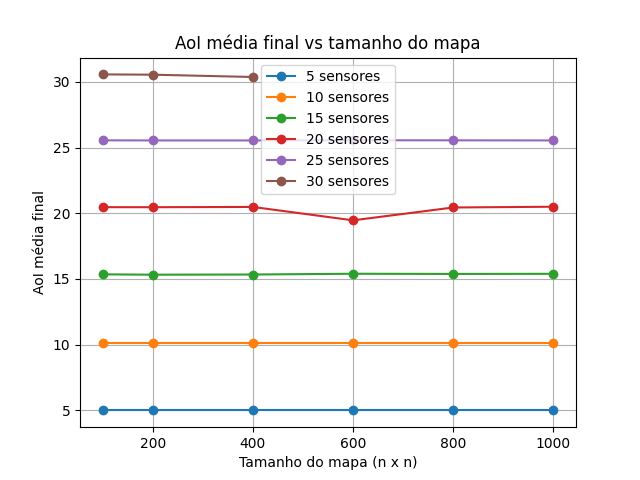
\includegraphics[width=\textwidth]{figs/anafi_aoi_vs_map.png}
    \caption{Parrot Anafi USA}
  \end{subfigure}
  \caption{AoI média final em função do tamanho do mapa.}
  \label{fig:aoi_vs_map}
\end{figure}

A distância total percorrida (Figura~\ref{fig:distance_vs_map}) acompanha o crescimento de $L$ em ambos os modelos e apresenta comportamento inverso em relação a $n_s$ em mapas grandes: mais sensores na mesma área reduzem as distâncias médias entre vizinhos, resultando em rotas mais curtas. Em mapas pequenos ($L \leq 200$\,m), esse efeito é menos pronunciado, pois mesmo com poucos sensores as distâncias entre nós já são curtas.

\begin{figure}[htbp]
  \centering
  \begin{subfigure}[t]{0.49\textwidth}
    \centering
    
\includegraphics[width=\textwidth]{figs/distance_vs_map.png}
    \caption{DJI Matrice 300 RTK}
  \end{subfigure}
  \hfill
  \begin{subfigure}[t]{0.49\textwidth}
    \centering
    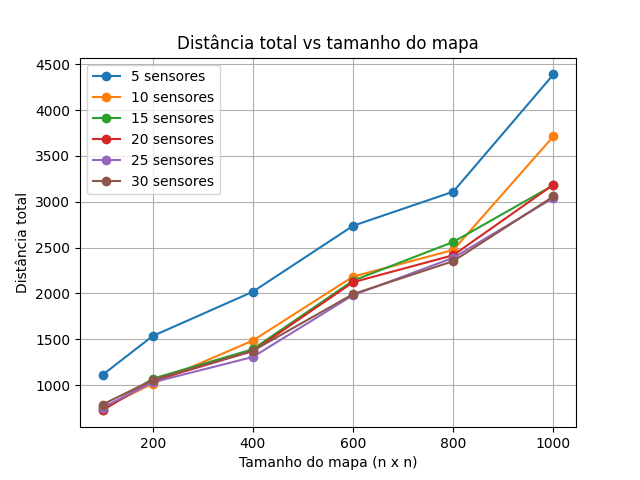
\includegraphics[width=\textwidth]{figs/anafi_distance_vs_map.png}
    \caption{Parrot Anafi USA}
  \end{subfigure}
  \caption{Distância total média em função do tamanho do mapa.}
  \label{fig:distance_vs_map}
\end{figure}

O consumo de energia (Figura~\ref{fig:energy_vs_map}) acompanha o aumento da área: quanto maior $L$, maiores as distâncias entre nós e, portanto, o custo energético de cada aresta. No DJI, o crescimento com $L$ é acentuado, com aparência aproximadamente exponencial na faixa avaliada, consequência de o custo por deslocamento crescer de forma super-linear com a distância percorrida em um único \textit{slot}. No Anafi, o crescimento também é pronunciado e apresenta dois saltos distintos, entre $L=400$ e $600$\,m e entre $L=600$ e $800$\,m. Observa-se ainda um comportamento não-monotônico em $L=1000$\,m: a energia do cenário com $n_s=5$ ($\approx$118\,kJ) supera a dos cenários com $n_s=10$ ($\approx$100\,kJ) e $n_s=15$ ($\approx$76\,kJ), pois, com apenas cinco sensores espalhados em 1000×1000\,m, as distâncias entre nós são maiores do que em cenários mais densos, tornando o roteamento mais custoso.

\begin{figure}[htbp]
  \centering
  \begin{subfigure}[t]{0.49\textwidth}
    \centering
    
\includegraphics[width=\textwidth]{figs/energy_vs_map.png}
    \caption{DJI Matrice 300 RTK}
  \end{subfigure}
  \hfill
  \begin{subfigure}[t]{0.49\textwidth}
    \centering
    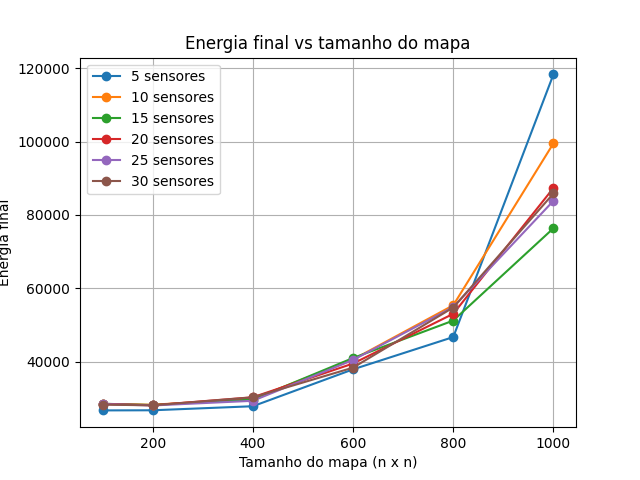
\includegraphics[width=\textwidth]{figs/anafi_energy_vs_map.png}
    \caption{Parrot Anafi USA}
  \end{subfigure}
  \caption{Energia média consumida em função do tamanho do mapa.}
  \label{fig:energy_vs_map}
\end{figure}

\subsection{Comparação com Heurísticas}
\label{sec:comparacao-heuristicas}

Para avaliar o desempenho do modelo de otimização (aqui chamado de MILP, resolvido via Gurobi) em relação a estratégias de baixo custo computacional, foram implementadas três heurísticas construtivas, todas avaliadas sobre os mesmos 36 cenários e as mesmas posições de sensores do Parrot Anafi USA, com 30 rodadas cada:

\begin{itemize}
\item \textbf{Nearest Neighbor (NN)}: a cada passo, o VANT visita o sensor viável (dentro do orçamento de bateria e \textit{slots}) mais próximo da posição atual.
\item \textbf{AoI-Greedy}: a cada passo, visita o sensor de maior AoI ainda viável, com desempate por proximidade. É a heurística mais alinhada ao objetivo de maximizar a AoI coletada.
\item \textbf{Score-Greedy}: a cada passo, visita o sensor de maior razão AoI/distância ainda viável, com desempate por proximidade. Pondera urgência e custo de deslocamento.
\end{itemize}

A Tabela~\ref{tab:cmp-heuristicas} apresenta as médias gerais das cinco métricas sobre todos os cenários. As Figuras~\ref{fig:cmp_all_collected_aoi} a~\ref{fig:cmp_all_energy} detalham, por métrica, o comportamento das quatro estratégias em função do tamanho do mapa, com os cenários separados por faixa de densidade em cada subfigura (a: 5 e 10 sensores; b: 15 e 20; c: 25 e 30).

\begin{table}[htbp]
  \centering
  \caption{Médias gerais das quatro estratégias sobre os 36 cenários (30 rodadas cada) -- Parrot Anafi USA. Para AoI coletada e sensores visitados, maior é melhor. Para AoI média final, energia e distância, menor é melhor.}
  \label{tab:cmp-heuristicas}
  \begin{tabular}{l r r r r}
    \toprule
    \textbf{Métrica} & \textbf{MILP} & \textbf{NN} & \textbf{AoI-Greedy} & \textbf{Score-Greedy} \\
    \midrule
    AoI coletada por rodada      & 309,7  & 145,4   & 298,5  & 300,5 \\
    AoI média final              & 17,8   & 127,2   & 29,5   & 28,5 \\
    Energia final (J)            & 44.943 & 48.711  & 64.571 & 57.738 \\
    Distância total (m)          & 1.933  & 1.272   & 1.719  & 1.502 \\
    Sensores visitados           & 8,33   & 8,22    & 8,19   & 8,24 \\
    \bottomrule
  \end{tabular}
\end{table}

A AoI coletada por rodada (Figura~\ref{fig:cmp_all_collected_aoi}) mede quanta informação desatualizada cada estratégia recolhe ao longo da missão. As heurísticas AoI-Greedy e Score-Greedy, construídas em torno do mesmo objetivo do MILP, aproximam-se muito do modelo ótimo: a AoI-Greedy fica a apenas $-3{,}6\%$ (298,5 contra 309,7) e a Score-Greedy a $-3{,}0\%$ (300,5). O NN coleta bem menos ($145,4$, menos da metade do MILP) e degrada sobretudo em mapas grandes com poucos sensores: nos cenários de 5 e 10 sensores (Figura~\ref{fig:cmp_collected_a}), sua curva despenca à medida que $L$ cresce, enquanto o MILP se mantém estável. Com o aumento da densidade (Figuras~\ref{fig:cmp_collected_b} e~\ref{fig:cmp_collected_c}), a diferença entre as estratégias diminui, pois há mais sensores próximos disponíveis para coleta.

\begin{figure}[htbp]
  \centering
  \begin{subfigure}{0.8\textwidth}
    \centering
    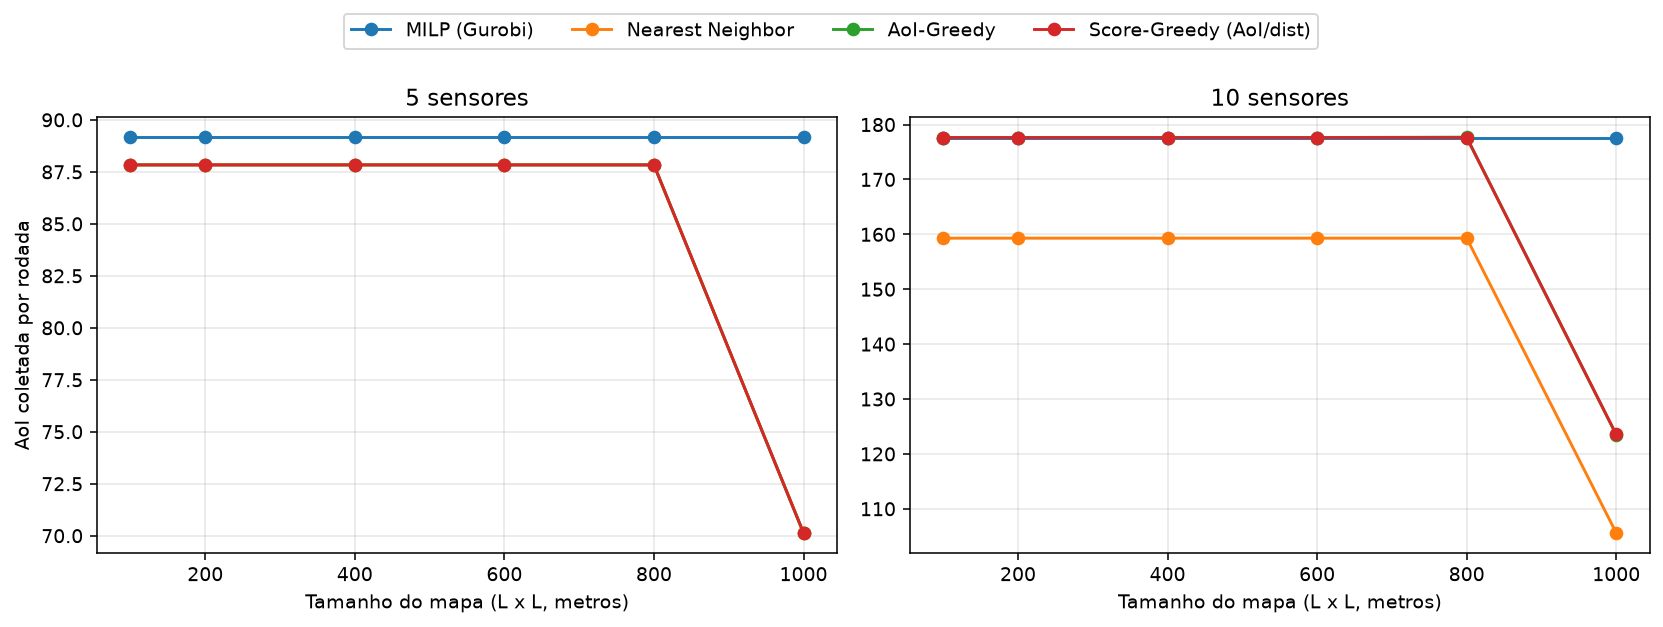
\includegraphics[width=\textwidth]{figs/cmp_all_collected_aoi_p1.png}
    \caption{5 e 10 sensores}
    \label{fig:cmp_collected_a}
  \end{subfigure}

  \begin{subfigure}{0.8\textwidth}
    \centering
    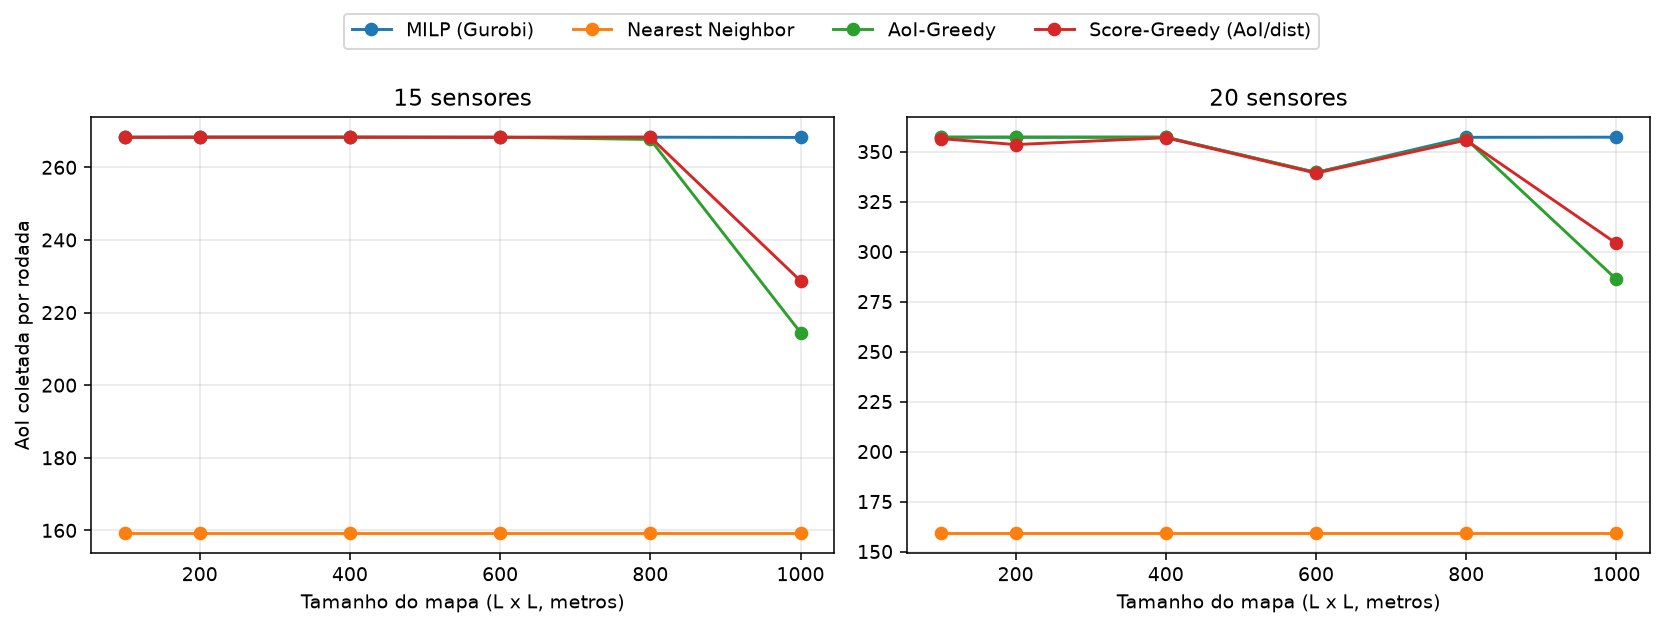
\includegraphics[width=\textwidth]{figs/cmp_all_collected_aoi_p2.png}
    \caption{15 e 20 sensores}
    \label{fig:cmp_collected_b}
  \end{subfigure}

  \begin{subfigure}{0.8\textwidth}
    \centering
    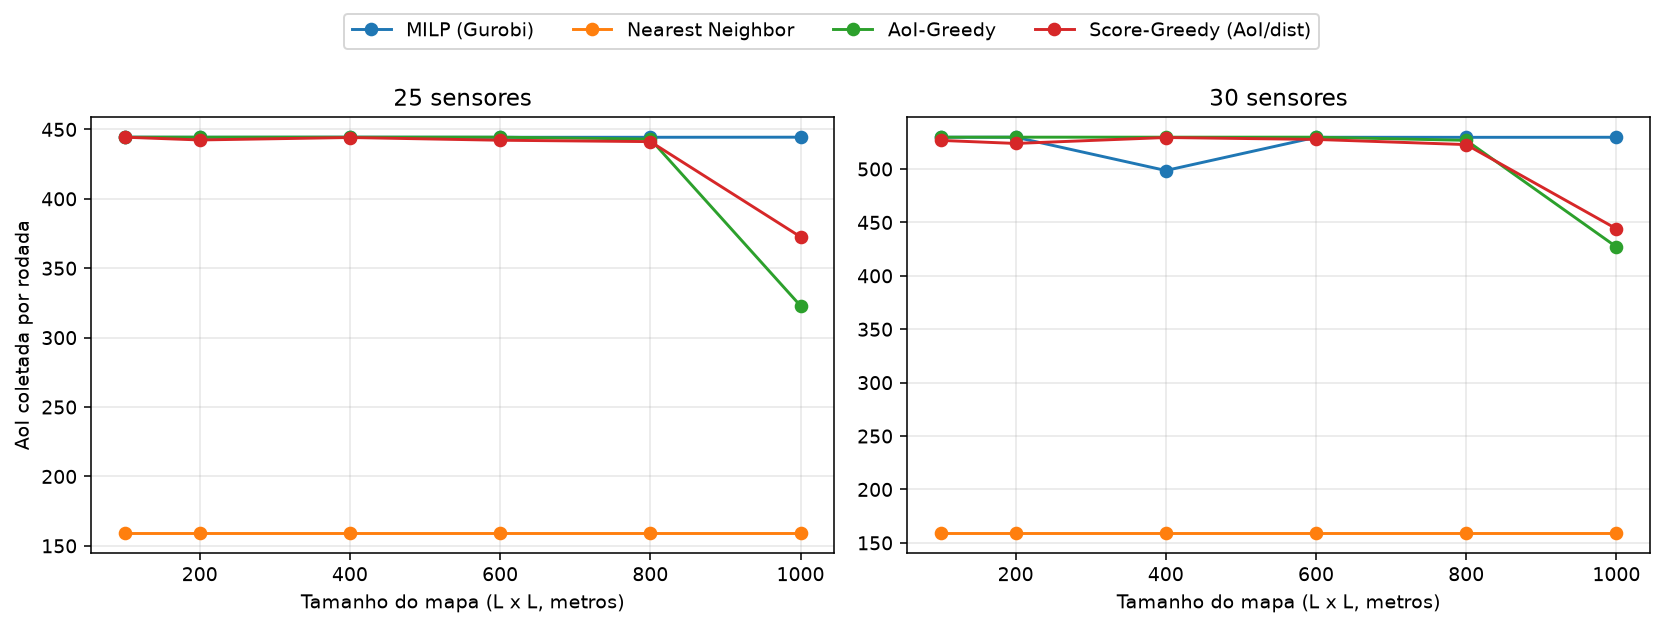
\includegraphics[width=\textwidth]{figs/cmp_all_collected_aoi_p3.png}
    \caption{25 e 30 sensores}
    \label{fig:cmp_collected_c}
  \end{subfigure}
  \caption{AoI coletada por rodada em função do tamanho do mapa, para as quatro estratégias.}
  \label{fig:cmp_all_collected_aoi}
\end{figure}

A AoI média final (Figura~\ref{fig:cmp_all_avg_final_aoi}) mede quão atualizados ficam os dados ao término da missão. O MILP entrega a menor idade residual (17,8), seguido de perto pela Score-Greedy (28,5) e pela AoI-Greedy (29,5), ambas cerca de $38$ a $40\%$ acima do MILP, porém muito melhores que o NN, que é o pior por larga margem (127,2). O contraste aparece com mais nitidez nos cenários de baixa densidade (Figura~\ref{fig:cmp_avg_a}), em que a curva do NN se descola das demais, refletindo sua incapacidade de manter a rede atualizada quando os sensores estão distantes.

\begin{figure}[htbp]
  \centering
  \begin{subfigure}{0.8\textwidth}
    \centering
    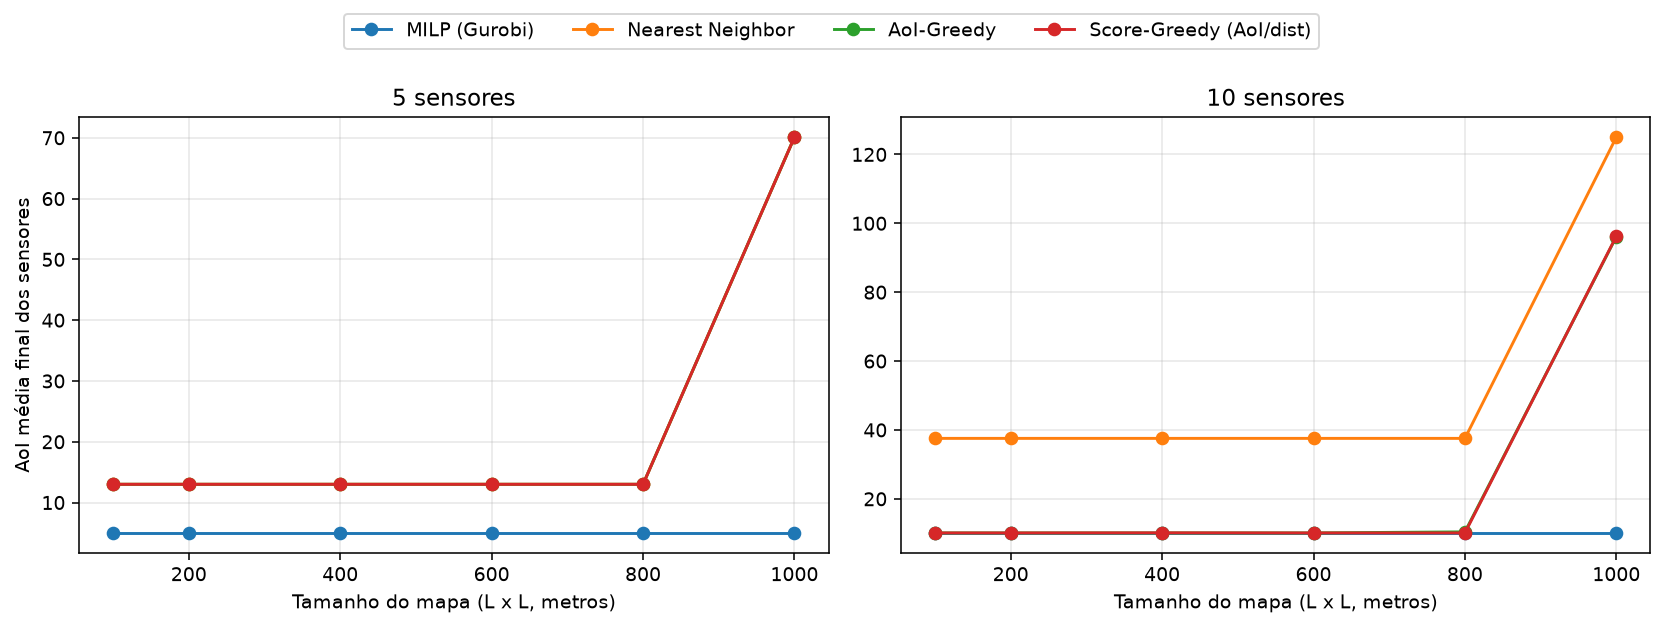
\includegraphics[width=\textwidth]{figs/cmp_all_avg_final_aoi_p1.png}
    \caption{5 e 10 sensores}
    \label{fig:cmp_avg_a}
  \end{subfigure}

  \begin{subfigure}{0.8\textwidth}
    \centering
    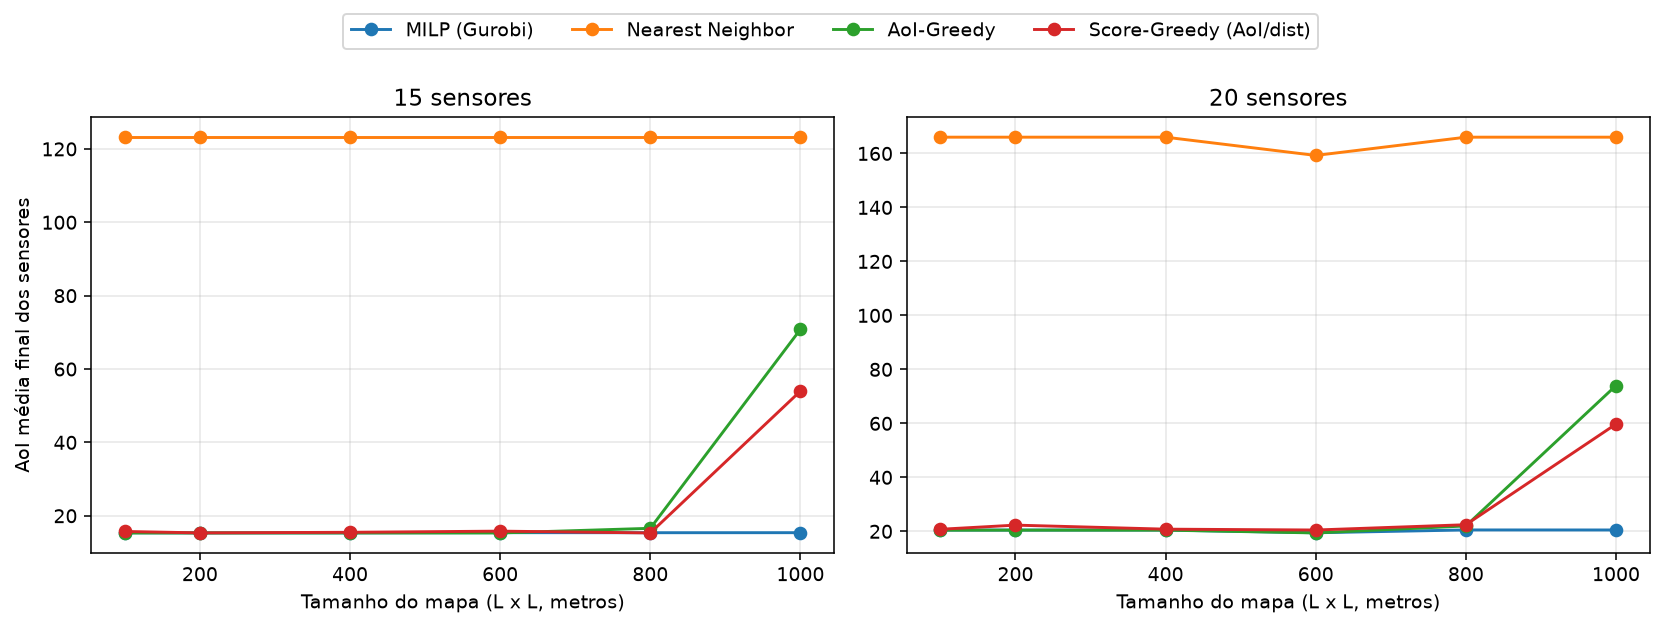
\includegraphics[width=\textwidth]{figs/cmp_all_avg_final_aoi_p2.png}
    \caption{15 e 20 sensores}
    \label{fig:cmp_avg_b}
  \end{subfigure}

  \begin{subfigure}{0.8\textwidth}
    \centering
    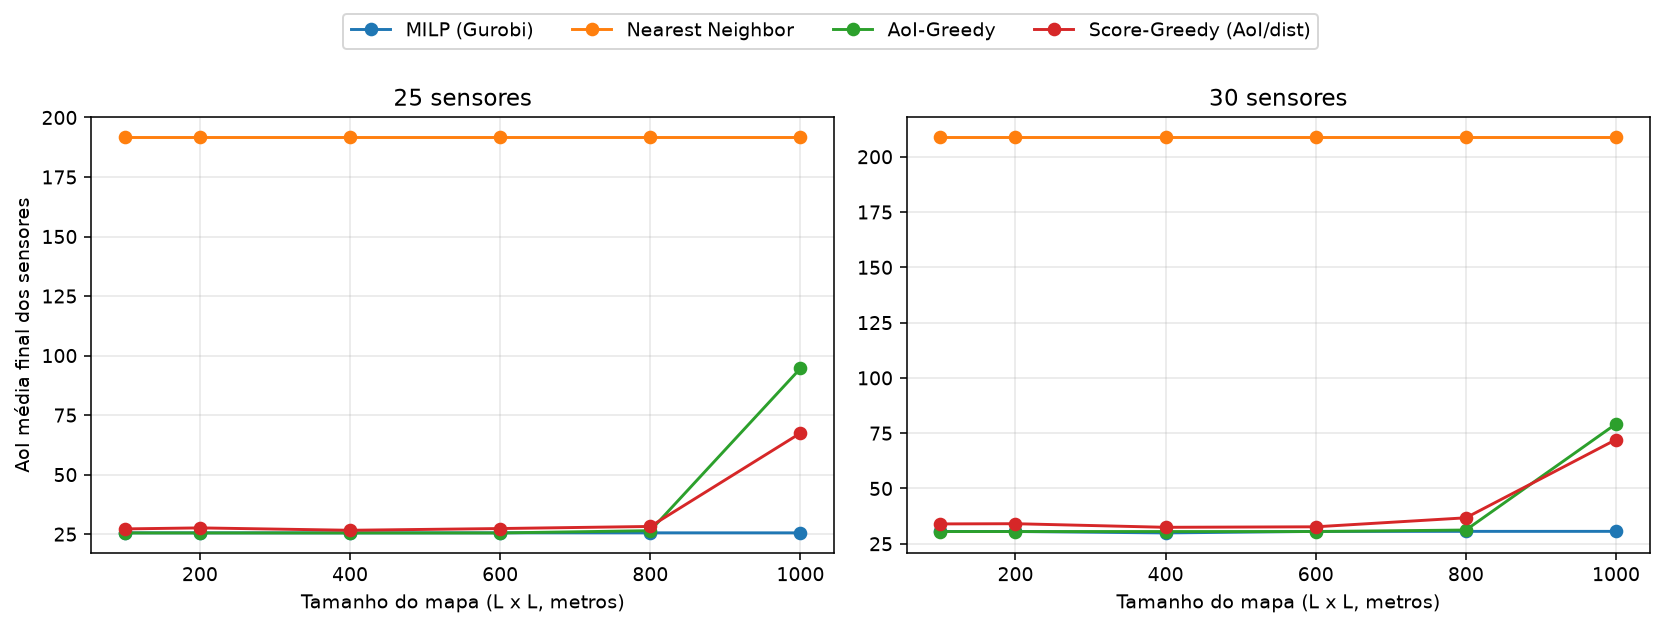
\includegraphics[width=\textwidth]{figs/cmp_all_avg_final_aoi_p3.png}
    \caption{25 e 30 sensores}
    \label{fig:cmp_avg_c}
  \end{subfigure}
  \caption{AoI média final dos sensores em função do tamanho do mapa, para as quatro estratégias.}
  \label{fig:cmp_all_avg_final_aoi}
\end{figure}

O consumo de energia (Figura~\ref{fig:cmp_all_energy}) evidencia o ponto fraco das heurísticas gulosas por AoI: a AoI-Greedy gasta $+43{,}7\%$ (64.571\,J contra 44.943\,J do MILP) e a Score-Greedy $+28{,}5\%$ (57.738\,J), pois maximizam a AoI sem ponderar adequadamente o custo do deslocamento. O NN consome pouco (48.711\,J, apenas $+7{,}7\%$ sobre o MILP), mas à custa de coletar pouco. A vantagem de ponderar a distância fica clara na comparação entre as duas gulosas: a Score-Greedy domina a AoI-Greedy, coletando essencialmente a mesma AoI ($+0{,}7\%$) com $-10{,}6\%$ de energia e $-12{,}6\%$ de distância. Em todas as estratégias, o consumo cresce de forma acentuada com $L$ (Figuras~\ref{fig:cmp_energy_a} a~\ref{fig:cmp_energy_c}).

\begin{figure}[htbp]
  \centering
  \begin{subfigure}{0.8\textwidth}
    \centering
    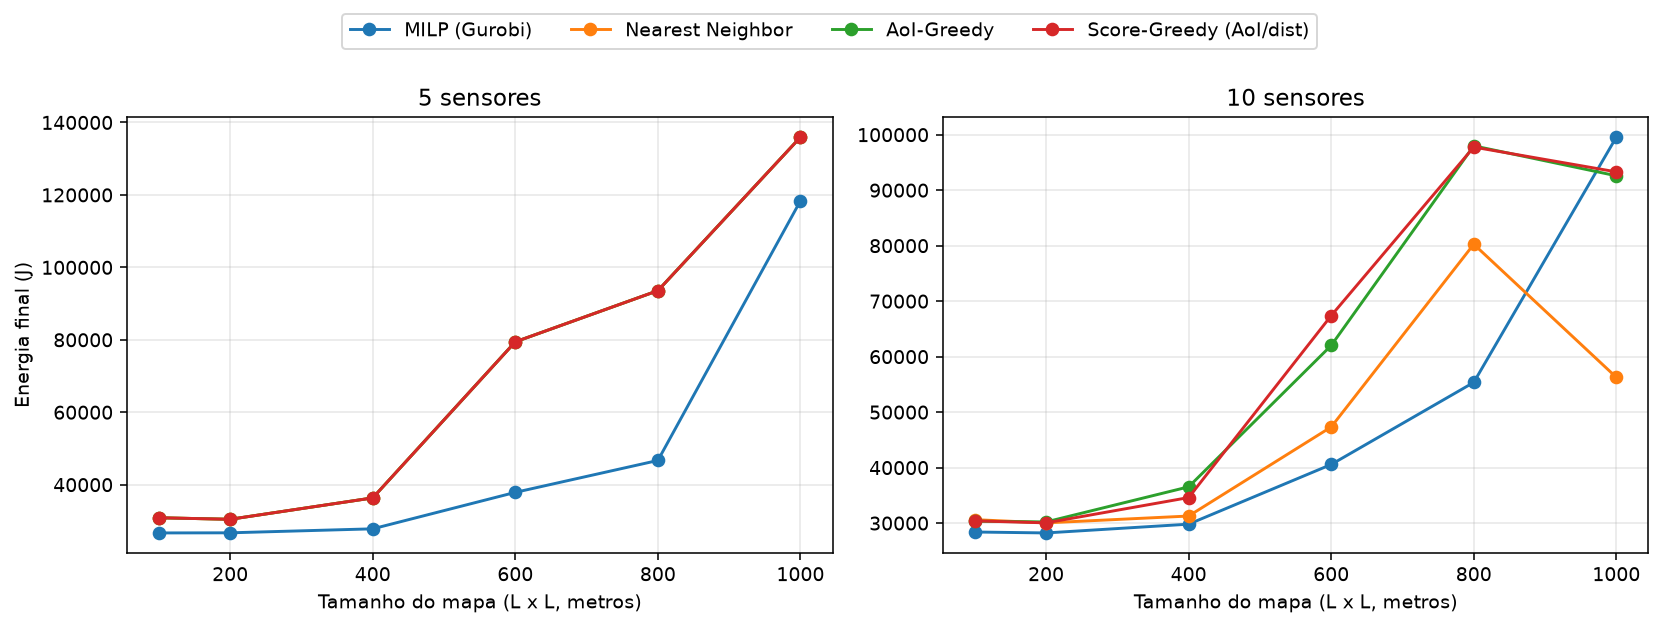
\includegraphics[width=\textwidth]{figs/cmp_all_energy_p1.png}
    \caption{5 e 10 sensores}
    \label{fig:cmp_energy_a}
  \end{subfigure}

  \begin{subfigure}{0.8\textwidth}
    \centering
    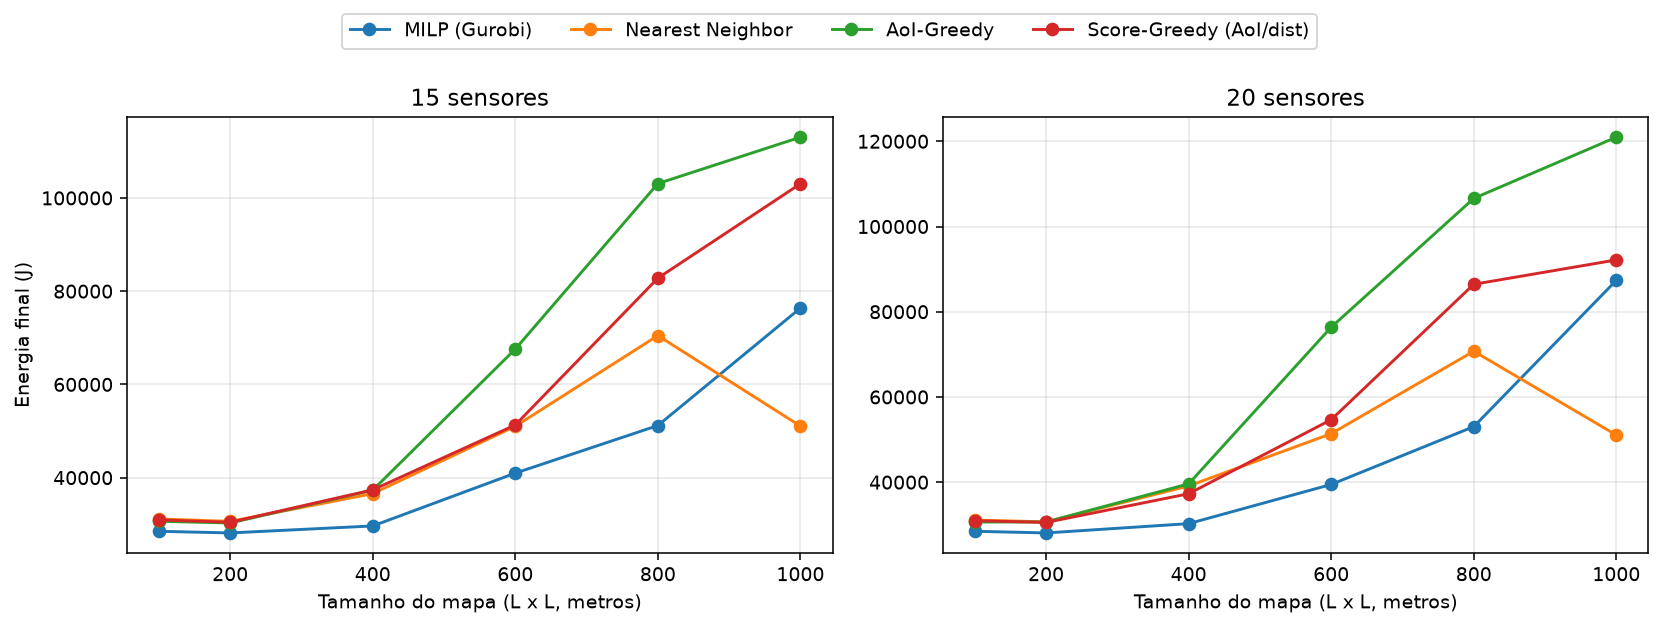
\includegraphics[width=\textwidth]{figs/cmp_all_energy_p2.png}
    \caption{15 e 20 sensores}
    \label{fig:cmp_energy_b}
  \end{subfigure}

  \begin{subfigure}{0.8\textwidth}
    \centering
    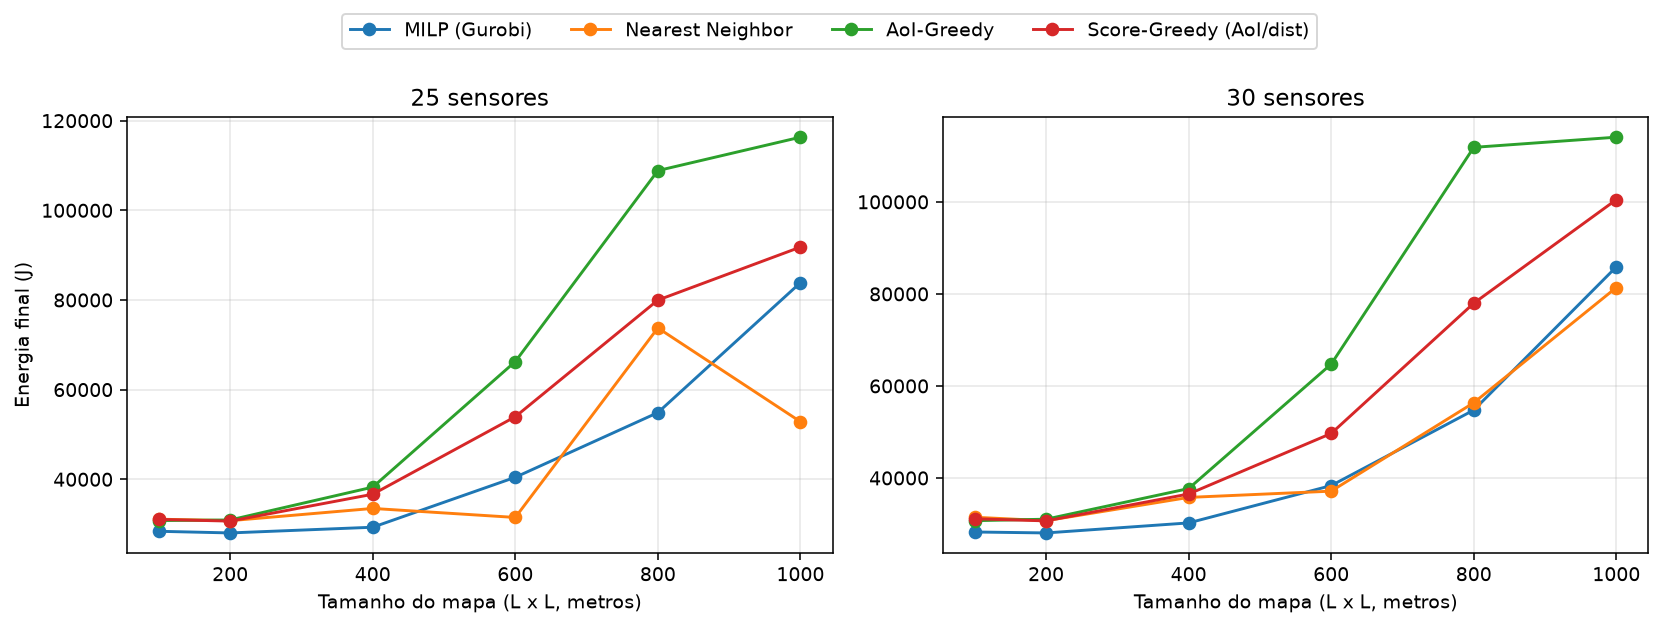
\includegraphics[width=\textwidth]{figs/cmp_all_energy_p3.png}
    \caption{25 e 30 sensores}
    \label{fig:cmp_energy_c}
  \end{subfigure}
  \caption{Energia final consumida em função do tamanho do mapa, para as quatro estratégias.}
  \label{fig:cmp_all_energy}
\end{figure}

Em síntese, cada heurística privilegia um aspecto isolado: o NN economiza energia mas coleta pouco e desatualiza a rede, enquanto as gulosas por AoI coletam quase tanto quanto o MILP, porém a um custo energético muito maior. A Score-Greedy é a melhor heurística do conjunto, dominando a AoI-Greedy e sendo a mais próxima do MILP, mas ainda assim permanece $28{,}5\%$ acima dele em energia. Isso evidencia o valor da formulação exata: por ser multiobjetivo lexicográfica (maximiza a AoI coletada e, em seguida, minimiza a energia entre as soluções de AoI ótima), o MILP é a única estratégia que alcança, ao mesmo tempo, a maior AoI coletada e o menor consumo energético.

\subsection{Variante com Revisitas}

Com base nos resultados do modelo base, investigou-se uma variante que relaxa a restrição de visita única por sensor: o modelo com revisitas (\textit{revisit}). Nessa configuração, o VANT pode visitar o mesmo sensor mais de uma vez durante uma missão, com o objetivo de coletar AoI adicional de sensores de alto valor nas rodadas em que a AoI acumulada é elevada.

\subsubsection{Implementação}
A modificação consiste na substituição da restrição de visita única (Equação~\eqref{eq:visita-unica}), $\sum_t v_{j,t} \leq 1$, por $\sum_t v_{j,t} \leq K$, onde $K$ é o número máximo de revisitas permitido por sensor por missão. O parâmetro $K$ é configurável via argumento de linha de comando (\texttt{--max-revisits}). Nos experimentos desta seção, adotou-se $K = 3$.

\subsubsection{Desafios computacionais}
A adoção de revisitas amplia consideravelmente o espaço de soluções viáveis do modelo MILP. Com $K = 3$, o número de combinações possíveis de padrões de visita cresce exponencialmente, tornando a exploração da árvore de \textit{branch-and-bound} pelo Gurobi significativamente mais custosa em memória. Em cenários com $n_s \geq 20$ e $L \geq 600$\,m, o processo de otimização chegou a consumir vários gigabytes de RAM, causando instabilidades no ambiente de execução.

Para contornar esses problemas, foram adotadas três medidas: (i) limitação do número de \textit{threads} do Gurobi a 2, reduzindo o paralelismo da exploração da árvore, (ii) ativação do parâmetro \texttt{NodefileStart = 0.5\,GB}, que instrui o solver a descarregar nós da árvore para disco ao atingir esse limite de memória RAM, e (iii) definição de \texttt{SoftMemLimit = 4\,GB}, que encerra a otimização de forma controlada e retorna a melhor solução encontrada até o momento quando o uso de memória ultrapassa esse valor. Adicionalmente, rodadas em que o solver não encontrou solução viável dentro do limite de tempo ou memória são registradas com métricas zeradas e AoI envelhecida normalmente, garantindo a consistência da cadeia de estado entre rodadas.

\subsubsection{Resultados e comparativo}
Os resultados do modelo com revisitas foram comparados com o modelo base para os mesmos 36 cenários, utilizando as mesmas posições de sensores e os mesmos parâmetros do Parrot Anafi USA.

A análise revela que a variante com revisitas \textbf{não trouxe melhora na qualidade da solução} em termos de AoI. Como mostra a Figura~\ref{fig:cmp_aoi_vs_map}, as curvas do modelo base e da variante com revisitas praticamente se sobrepõem em todas as faixas de densidade, dos cenários esparsos (Figura~\ref{fig:rev_aoi_a}) aos mais densos (Figura~\ref{fig:rev_aoi_c}). O mapa de variação percentual da AoI (Figura~\ref{fig:delta_aoi}) confirma o quadro: a AoI média final permaneceu estatisticamente equivalente ao modelo base em praticamente todos os cenários, com variações menores que $\pm 3\%$, dentro da margem de ruído das 30 rodadas.

\begin{figure}[htbp]
  \centering
  \begin{subfigure}{0.8\textwidth}
    \centering
    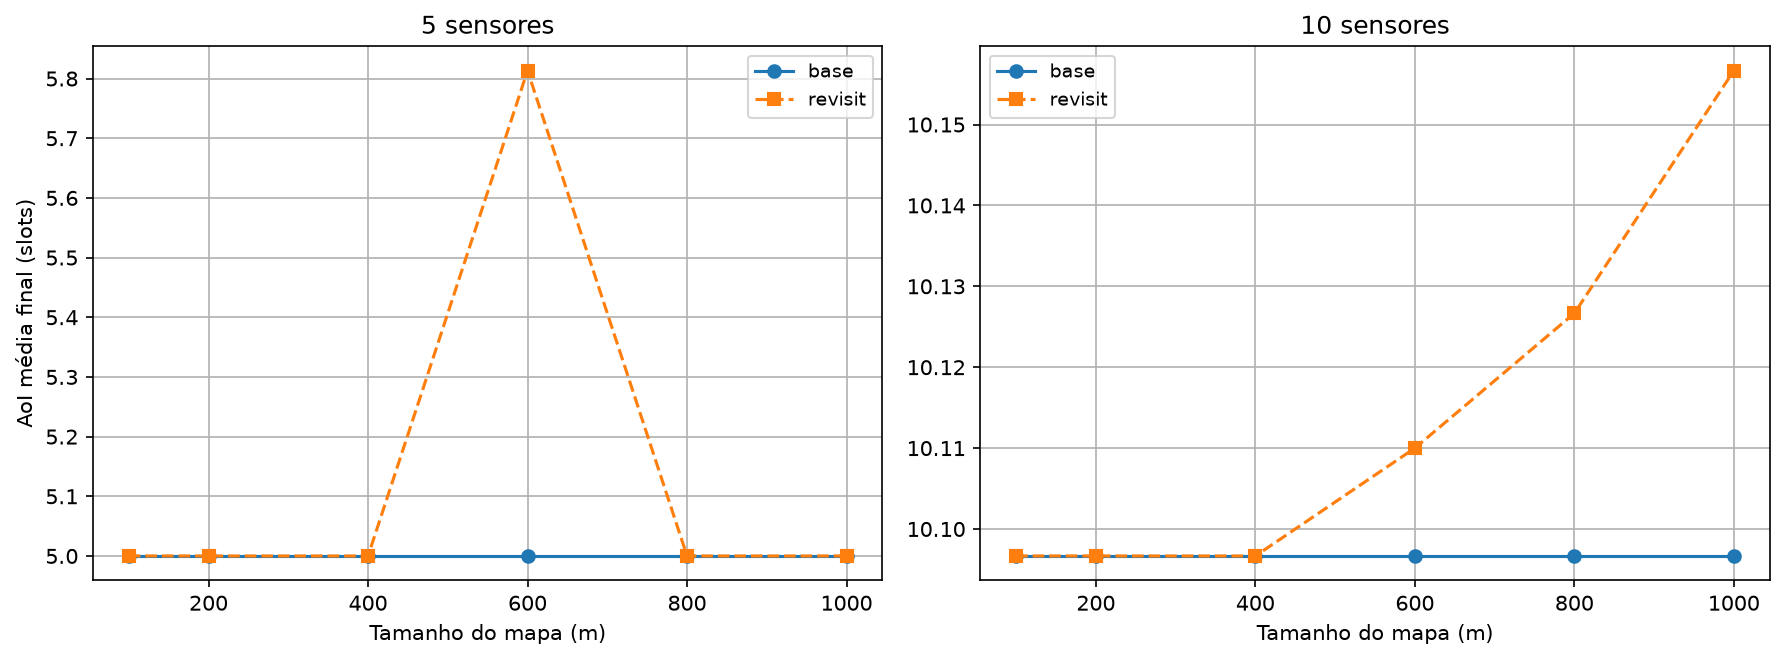
\includegraphics[width=\textwidth]{figs/cmp_aoi_vs_map_p1.png}
    \caption{5 e 10 sensores}
    \label{fig:rev_aoi_a}
  \end{subfigure}

  \begin{subfigure}{0.8\textwidth}
    \centering
    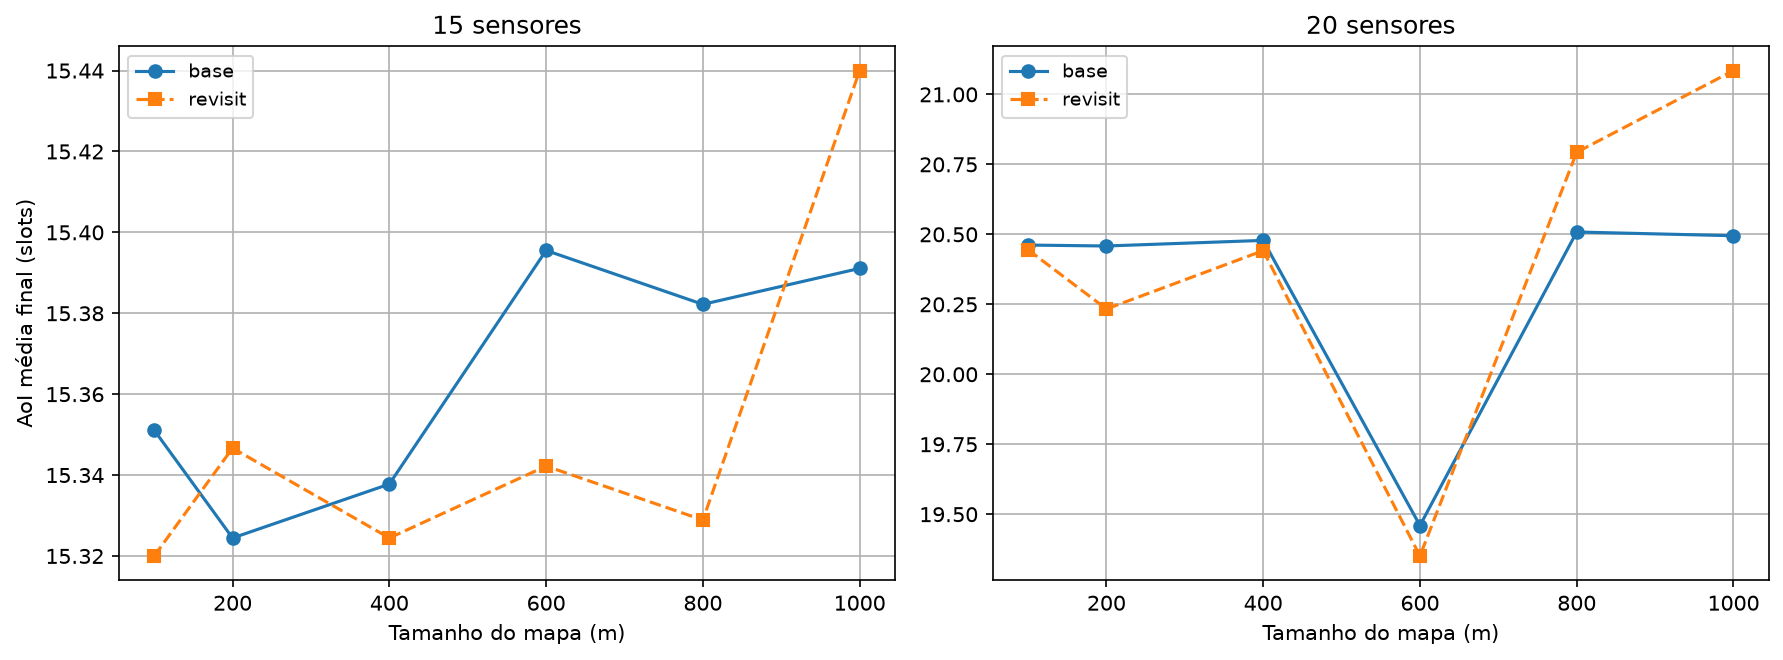
\includegraphics[width=\textwidth]{figs/cmp_aoi_vs_map_p2.png}
    \caption{15 e 20 sensores}
    \label{fig:rev_aoi_b}
  \end{subfigure}

  \begin{subfigure}{0.8\textwidth}
    \centering
    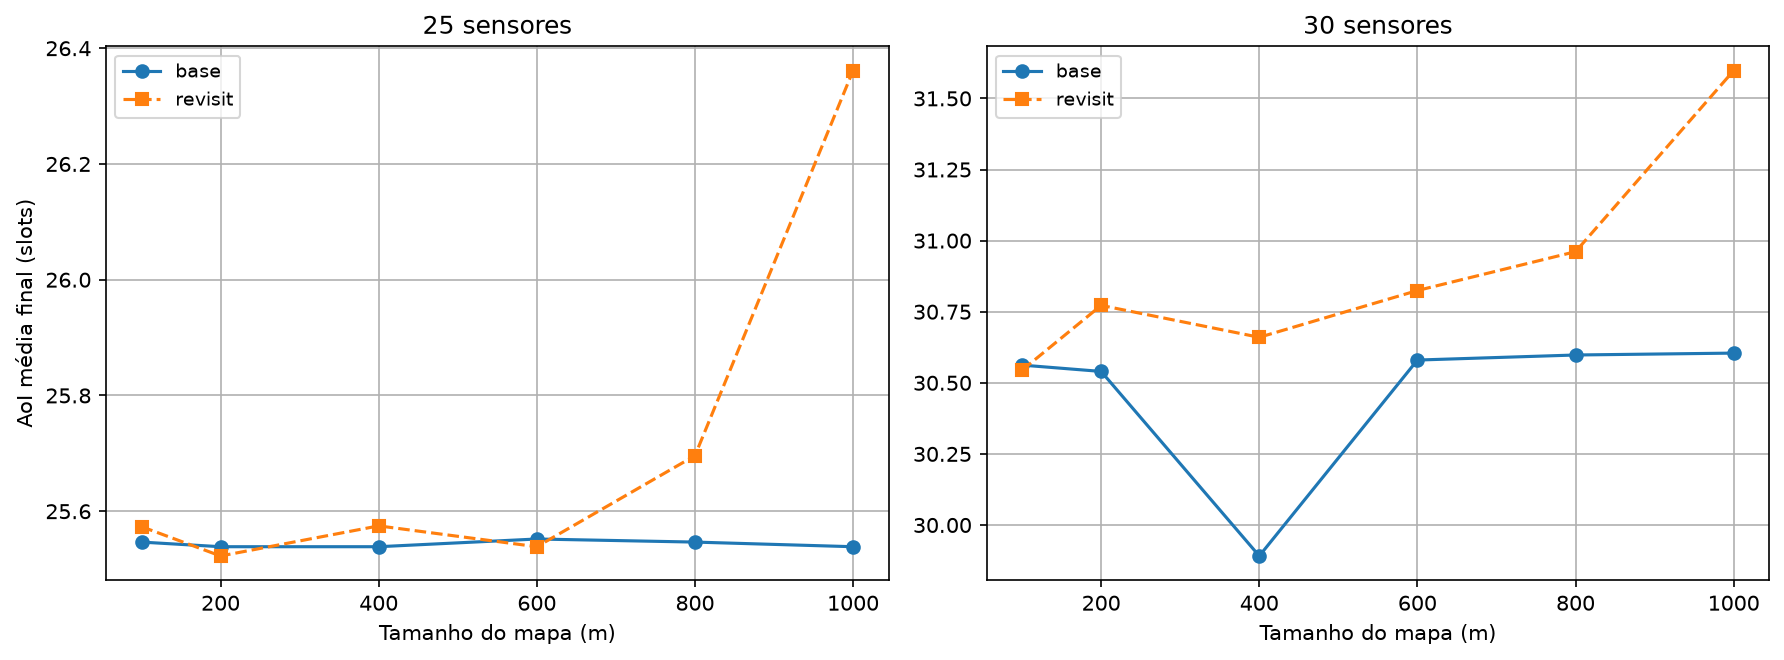
\includegraphics[width=\textwidth]{figs/cmp_aoi_vs_map_p3.png}
    \caption{25 e 30 sensores}
    \label{fig:rev_aoi_c}
  \end{subfigure}
  \caption{AoI média final: comparativo entre o modelo base e a variante com revisitas ($K=3$).}
  \label{fig:cmp_aoi_vs_map}
\end{figure}

Em contrapartida, o consumo energético aumentou substancialmente com as revisitas (Figura~\ref{fig:cmp_energy_vs_map}). Para mapas pequenos ($L \leq 200$\,m), o acréscimo foi modesto ($+3$ a $+6\%$), mas cresce fortemente com a área: entre $+33\%$ e $+45\%$ para $L=400$\,m e entre $+108\%$ e $+189\%$ para $L \geq 600$\,m, efeito que se acentua dos cenários de baixa densidade (Figura~\ref{fig:rev_energy_a}) aos de alta (Figura~\ref{fig:rev_energy_c}) e que o mapa de variação da energia (Figura~\ref{fig:delta_energy}) resume. Em vários cenários com $L \geq 600$\,m, a energia da variante ultrapassou $100$\,kJ, aproximando-se do limite de bateria de $141$\,kJ.

\begin{figure}[htbp]
  \centering
  \begin{subfigure}{0.8\textwidth}
    \centering
    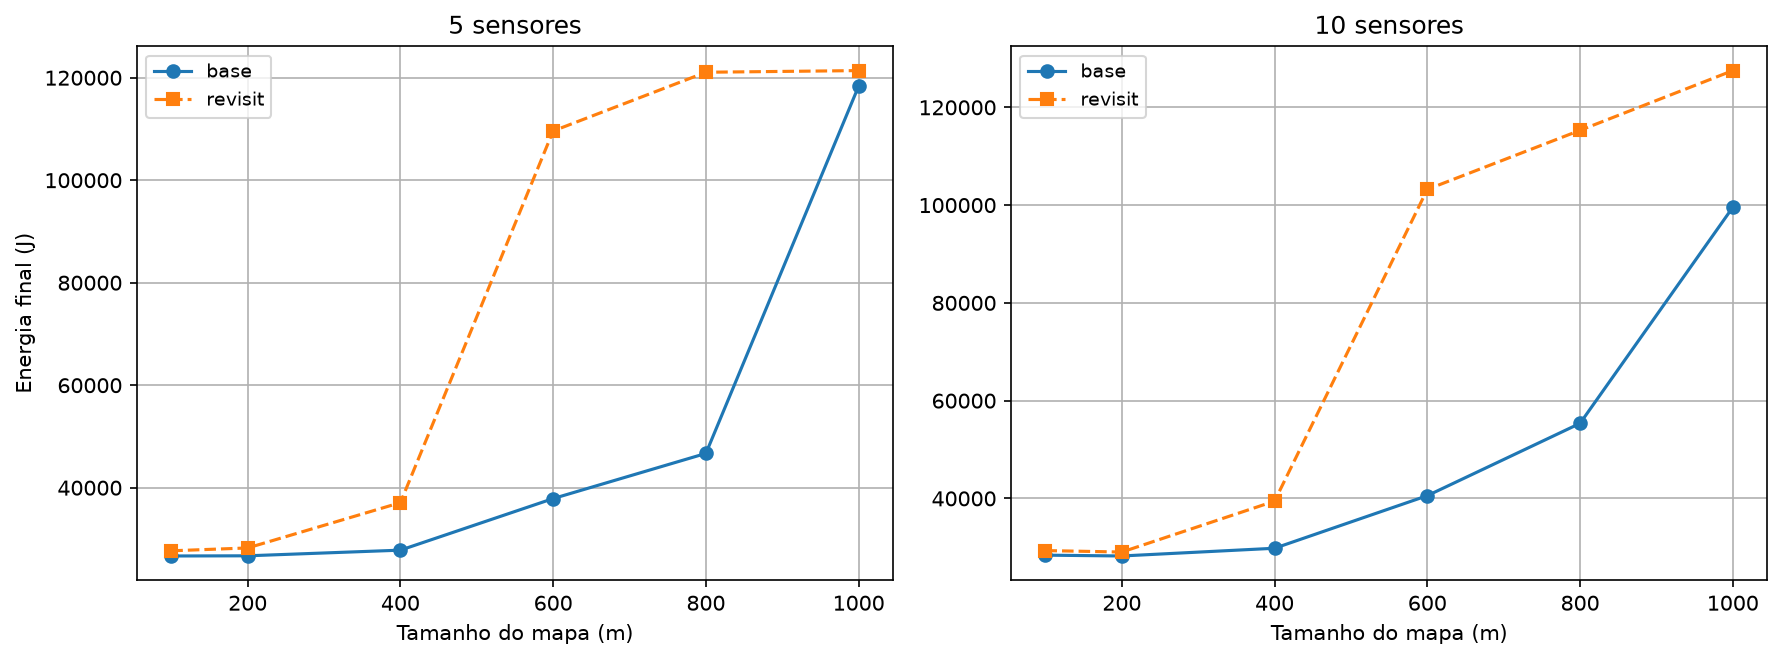
\includegraphics[width=\textwidth]{figs/cmp_energy_vs_map_p1.png}
    \caption{5 e 10 sensores}
    \label{fig:rev_energy_a}
  \end{subfigure}

  \begin{subfigure}{0.8\textwidth}
    \centering
    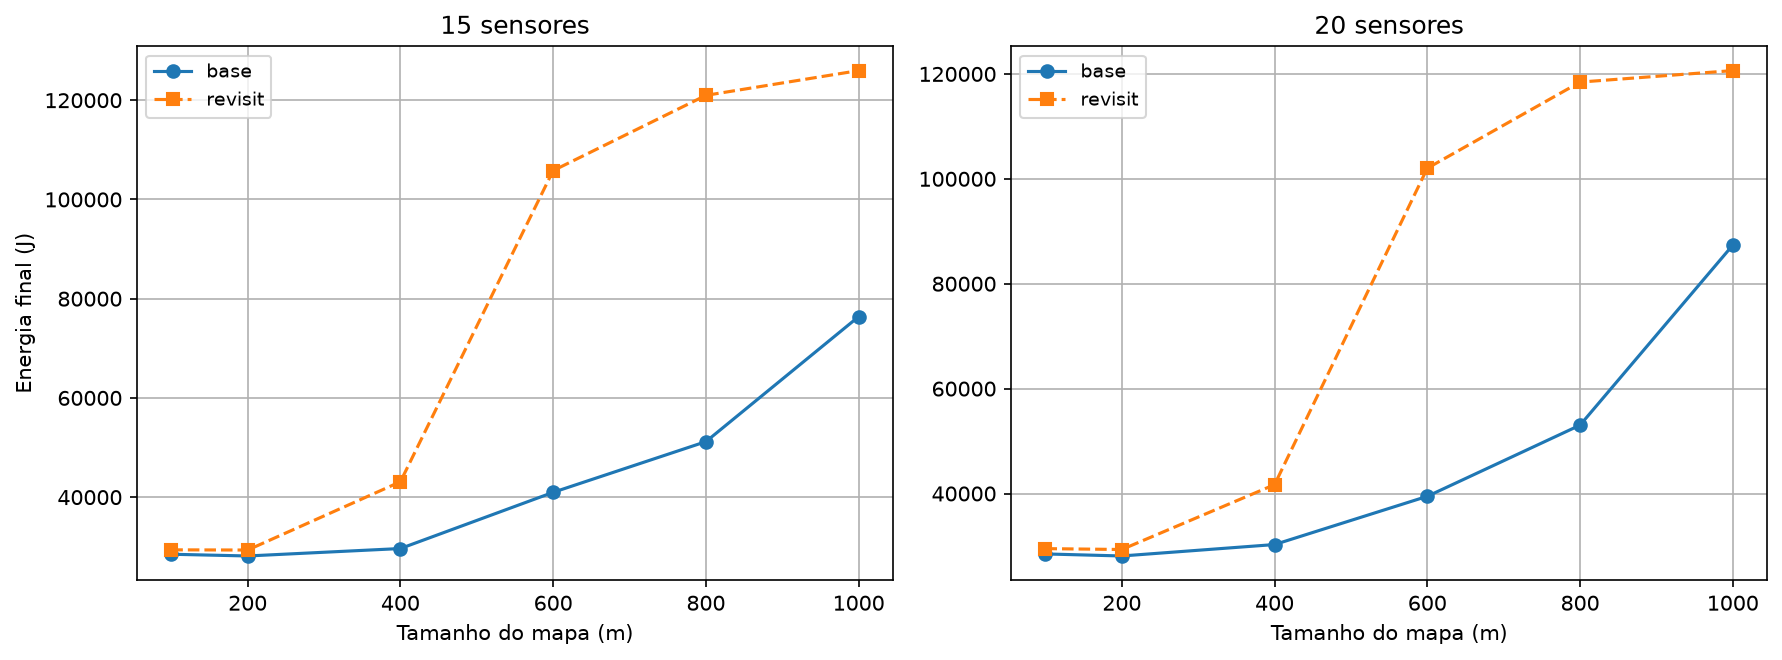
\includegraphics[width=\textwidth]{figs/cmp_energy_vs_map_p2.png}
    \caption{15 e 20 sensores}
    \label{fig:rev_energy_b}
  \end{subfigure}

  \begin{subfigure}{0.8\textwidth}
    \centering
    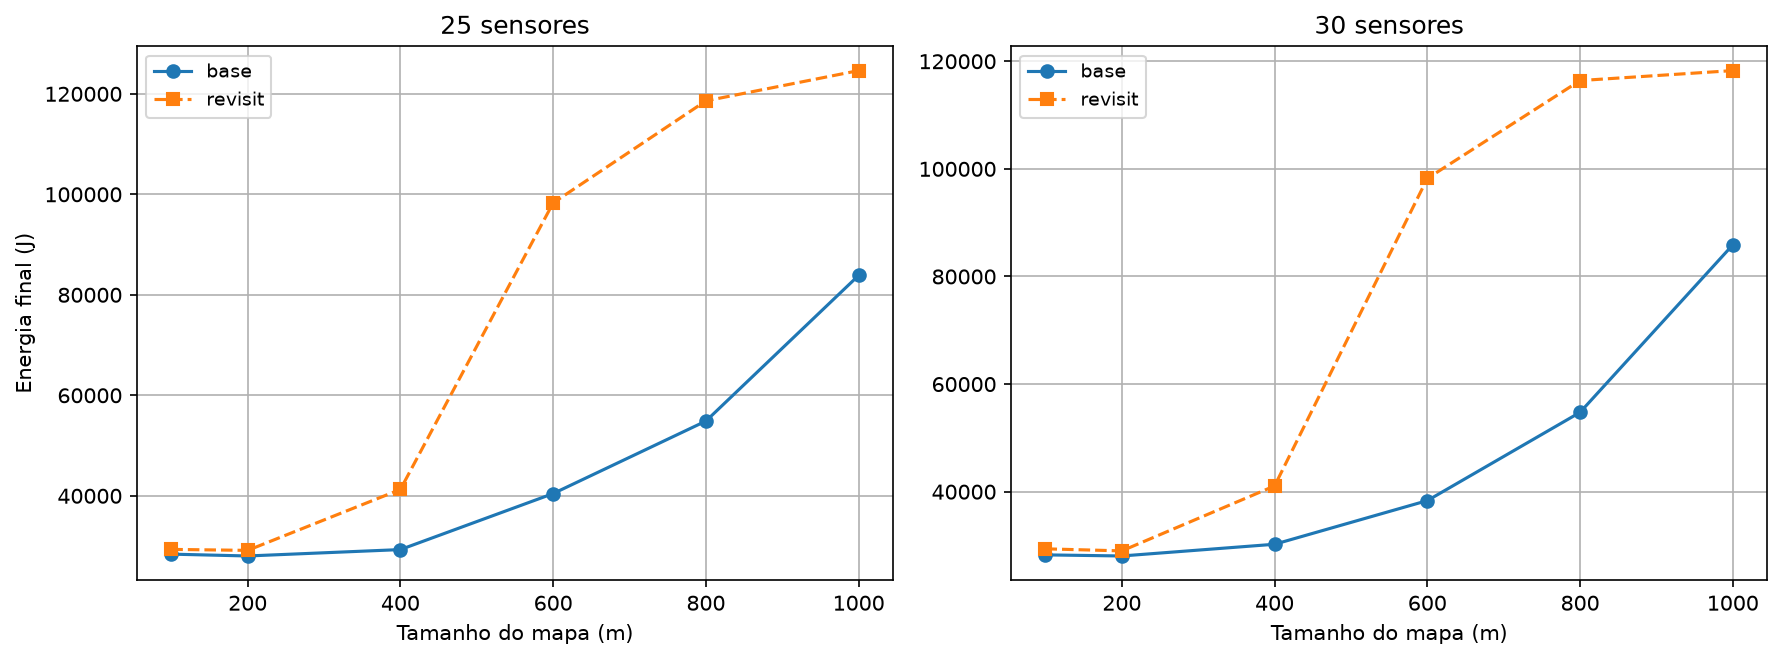
\includegraphics[width=\textwidth]{figs/cmp_energy_vs_map_p3.png}
    \caption{25 e 30 sensores}
    \label{fig:rev_energy_c}
  \end{subfigure}
  \caption{Energia média consumida: comparativo entre o modelo base e a variante com revisitas ($K=3$).}
  \label{fig:cmp_energy_vs_map}
\end{figure}

\begin{figure}[htbp]
  \centering
  \begin{subfigure}[t]{0.49\textwidth}
    \centering
    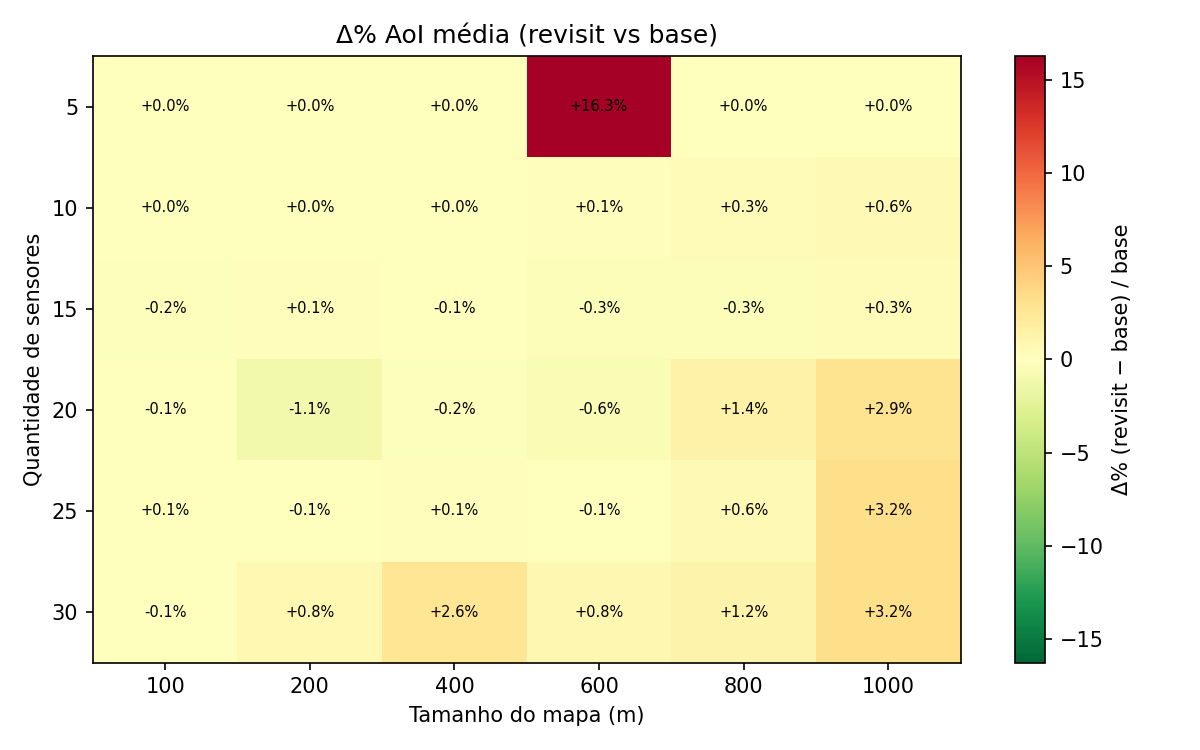
\includegraphics[width=\textwidth]{figs/delta_aoi_heatmap.png}
    \caption{AoI média final}
    \label{fig:delta_aoi}
  \end{subfigure}
  \hfill
  \begin{subfigure}[t]{0.49\textwidth}
    \centering
    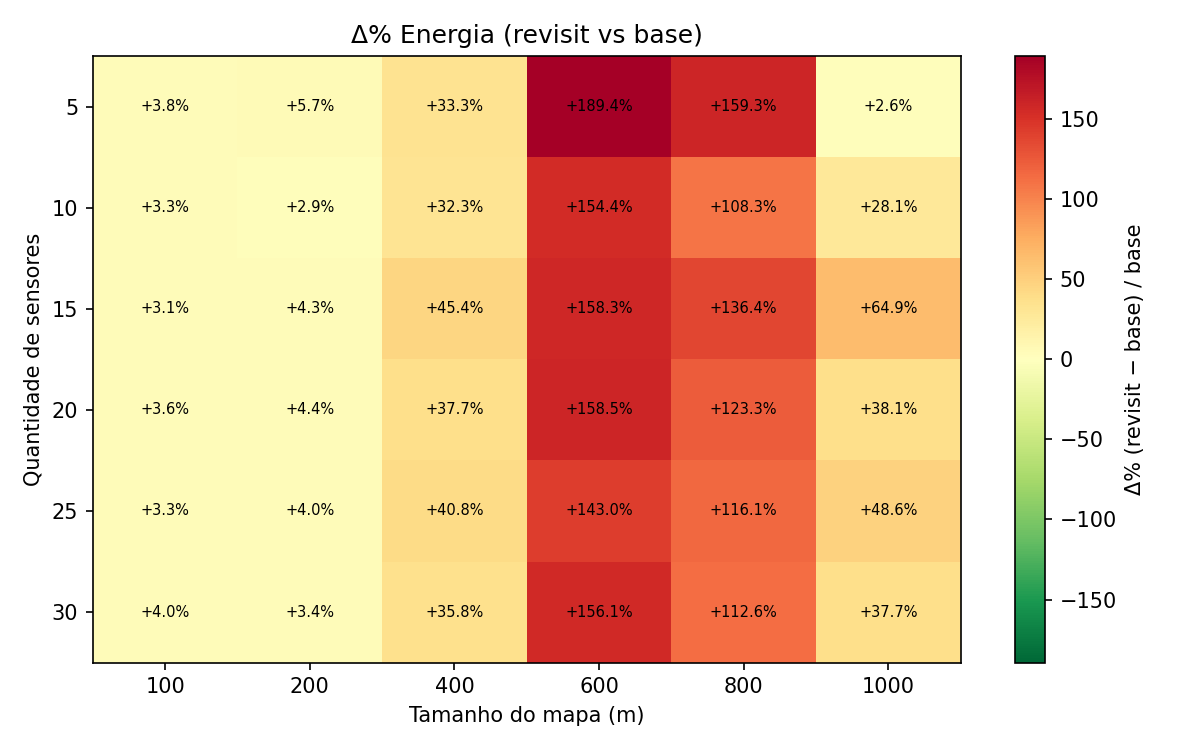
\includegraphics[width=\textwidth]{figs/delta_energy_heatmap.png}
    \caption{Energia consumida}
    \label{fig:delta_energy}
  \end{subfigure}
  \caption{Variação percentual (revisit $-$ base) / base entre a variante com revisitas e o modelo base. Valores positivos indicam piora (aumento).}
  \label{fig:delta_heatmaps}
\end{figure}

Esse comportamento pode ser explicado pela natureza do modelo de otimização: ao permitir revisitas, o solver passa a incluir trajetórias em que o VANT retorna a sensores já visitados para coletar, em um \textit{slot} posterior, a AoI que eles voltaram a acumular desde a visita anterior, mas esse ganho marginal de AoI não compensa o custo energético do deslocamento adicional. Com $K=3$, o orçamento de tempo pairado disponível é distribuído em menos sensores distintos, reduzindo a diversidade de coleta e, consequentemente, sem benefício líquido para a AoI média da rede.

Conclui-se que, para a configuração estudada ($K=3$, 20 slots de 10\,s, Parrot Anafi USA), a restrição de visita única é uma escolha eficiente: ela força o otimizador a diversificar as visitas, obtendo qualidade de AoI equivalente a um custo energético significativamente menor.

\subsection{Escala espacial e o papel das heurísticas}
\label{sec:escala-heuristicas}

Os experimentos apresentados restringiram-se a áreas de até $1000\times1000$\,m. Essa escolha decorre da discretização adotada no modelo de energia (Capítulo~\ref{sec:modelagem}): como cada transição entre nós é concluída em um único \textit{slot} de duração fixa $\Delta t = 10$\,s, áreas maiores implicariam velocidades nominais irrealistas e, com frequência, um custo energético por deslocamento superior à própria capacidade da bateria, tornando o cenário fisicamente inviável sob essa parametrização.

As heurísticas construtivas, por si só, não são o fator limitante: elas podem ser executadas em áreas maiores sem dificuldade. Para tornar tais áreas energeticamente viáveis, entretanto, seria necessário aumentar a duração do \textit{slot} $\Delta t$, permitindo velocidades menores e um custo de deslocamento compatível com a bateria. Esse ajuste, porém, altera a base temporal do experimento e inviabiliza a comparação direta com os cenários menores, que adotam $\Delta t = 10$\,s. Além disso, um $\Delta t$ maior é contraproducente no cenário menor: como o custo do voo pairado cresce linearmente com $\Delta t$, o consumo mínimo da missão, mesmo sem deslocamentos, pode se aproximar ou exceder a capacidade da bateria, dificultando a obtenção de soluções viáveis. Não havendo uma parametrização única de $\Delta t$ que permita comparar de forma justa cenários de escalas muito distintas, optou-se por não apresentar resultados de heurísticas em áreas maiores.

Cabe destacar, ainda, o custo computacional do modelo exato. A demanda de memória do resolvedor cresce rapidamente com o tamanho da instância. Na prática, os cenários de $1000\times1000$\,m com $20$ ou mais sensores exigiram consumo de memória próximo aos limites do ambiente de teste, chegando a comprometer a estabilidade da máquina durante a otimização. Esse comportamento reforça que, à medida que a instância cresce, a resolução exata torna-se progressivamente mais custosa não apenas em tempo, mas também em recursos de hardware.

Ainda assim, mesmo nos cenários avaliados, as heurísticas constituem uma alternativa prática ao modelo exato: enquanto o MILP requer o resolvedor Gurobi e pode esgotar o limite de tempo e a memória disponível, as heurísticas produzem uma solução em uma fração do tempo e com uso de recursos muito menor, atingindo qualidade de coleta próxima à do modelo ótimo (Seção~\ref{sec:comparacao-heuristicas}). Uma solução mais adequada para abranger áreas maiores sem comprometer a comparabilidade seria reformular o modelo com restrições explícitas de velocidade, desacoplando a velocidade de voo da duração do \textit{slot}. Essa direção é retomada como trabalho futuro (Capítulo~\ref{cap:conclusao}).
